\documentclass[a4paper,10pt]{article}
\usepackage[utf8]{inputenc}
\usepackage[pdftex]{graphicx}   
\usepackage{float}

%opening
\title{A Genome Assembly Graph \\
    \smallskip
    \large{DA3018} \\
    \smallskip
    \large{Spring 2019}}
\author{Anton Stråhle \\ 
    Jan Alexandersson \\
    Fredrika Lundahl}

\date{}    

\setlength{\parindent}{0pt}

\newcommand\bref[1]{[\ref{#1}]}

\begin{document}

\maketitle

\section{Introduction}

In this project we examine data consisting of genome assemblies of norwegian spruces. The data set is made up of the starting and ending indexes of the overlap between so called contigs. We let the contigs represent some nodes in a graph whilst the overlap between two contigs creates an edge, which gives us some genome assembly graph which henceforth will be referred to simply as the graph. 

\medskip

Using this graph we are to find the average degree and the degree distribution. Furthermore we also wish to observe the number of disconnected subgraphs of the genome assembly graph whilst also observing the distribution of the sizes of the subgraphs. 

\medskip

It turns out to be difficult to perform more precise operations on data of this size and as a result we also wish to create some partition method which given the initial graph returns some set of subgraphs containing less than 1000 contigs each. 

\section{Creating the Graph}

In order to create our actual graph we have to translate the actual data set to nodes and edges. In the data set we are given some identifiers for the contigs in question and information regarding their overlap. If an overlap exists between the contigs we create and edge between them. There is however one exception to this rule which is that an edge is not created if one of the contigs is a subsequence of the other. The reason for this is that the occurences of such subsequences is the outcome of containment.

\medskip

Using the set of rules determined in the paragraph above we created a converter which given the input data returns the desired graph. 

\medskip

Running the converter from the data file in order to create the graph worked without problem when using smaller test files but we ran into problems when running it with the whole data set. We got a garbage collection error and after some searching on the Intenet we realised we could just allow Java to use more RAM (Java uses 4G per default) and after giving Java 8G RAM to work with the program ran without error. We reasoned that this is a viable solution as computers nowadays generally have access to at least 8G RAM. 
If we can simply give Java more access to RAM then this solution is the most natural whilst also the being the quickest. So, we run the program in Unix using the line "java -Xmx8G DataToGraphConverter ../overlaps.m4", where the flag -Xmx8G specify how much RAM we we give Java access to.

\medskip

When examining the data in order to create our convereter we ovbiosuly could not examine the file as a whole due to its size. To bypass this issue we simply used the unix commands ''more'' ans ''less'' in order to examine the data page by page. In the early stages we also needed smaller test files to work with, for this we used the function "sed" to select an interval of lines from the file and create a new file with those. 

\subsection{Graph Representation}

In this project we have choosen to represent our graph using a so called adjacency list. The reasoning behind this is that the useage of an adjacency list holds several advantages compared to representations such as the adjacency matrix. Since the graph will be far from complete we would have a lot of zeros in our matrix which would both occupy more memory and slow down operations on the matrix. By using an adjacency list we avoid these issues and as a result use less memory and get faster operations. It is also preferable to use an adjacency list since it is very easy to derive the degree distribution from it. The only real advantage which an adjacency matrix has over a list is that its far quicker when you want to examine whether or not and edge exists between two nodes. Since this is not something that we have to do in this project it is clear that the adjacency list is far superior to the matrix. 

\section{Degree Distribution Prior to Partitioning}

In order to determine the degree distribution of our graph we simply used the nice functionality of the adjacency list by taking the sizes of each individual list of neighbors. Prior to the partitioning of the graph we were left with the following distribution.
\begin{figure}[H]
	\centering
	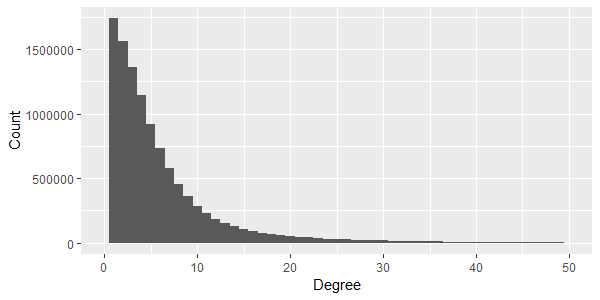
\includegraphics[width=0.85\linewidth]{degreesprior.png}
	\caption{Degree distribution before partitioning}
	\label{fig:degprior}
\end{figure}
As can be seen in Figure \bref{fig:degprior} we have a large number of nodes with degrees of reasonable level. There are however some nodes with degrees that exceed 100 which according to our knowledge should be impossible. When performing our partitions these nodes will be the first to be removed due to simply being unrealistic. In the figure we choose to exclude the representation of all nodes with degrees of 50 due to their rarity compared to those of lesser degree. The inclussion of these would alse stretch out the graph significantly which would make the results of smaller degrees more difficult to interpret. 

\section{Distribution of Disconnected Subgraphs Prior to Partitioning}

In order to determine the number of disconnected subgraphs and the sizes of these in our graph we implement a Flood Fill algorithm. The Flood Fill algorithm works by choosing some random node and give it some colour. Then all the neighbors of that node are coloured with the same colour. The procedure is repeated on their neighbors and so on untill there are no nodes left to colour. When this occurs we choose some non-coloured node and give it some different colour. This is repeated until there are no more nodes to colour. The number of different of colours in our graph is the number of disconnected subgraphs whilst the nodes of each colour gives us the size distribution of the subgraphs. In the actual algorithm we let the colours be represented by integers meaning that nodes belong to subgraph $0,1,2,...$. The distribution of the sizes of the subgraphs looks as follows before we partition the graph further.

\begin{figure}[H]
	\centering
	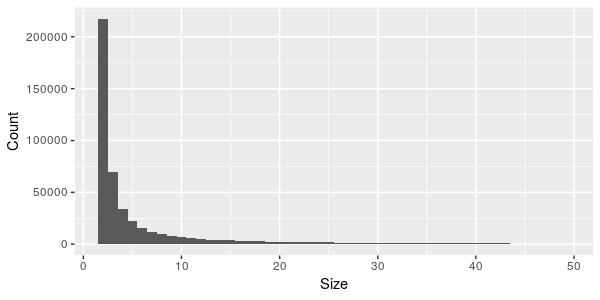
\includegraphics[width=0.85\linewidth]{sizesprior.png}
	\caption{Size distribution of the disconnected subgraphs before partitioning}
	\label{fig:sizeprior}
\end{figure}

In Figure \bref{fig:sizeprior} we have choosen to examine the sizes of the smaller subgraphs. There exists some disconnected subgraphs with degrees over 50 but they are very few compared to the many smaller ones. We note from the figure that the subgraphs of size $2$ are extremely frequent, meaning that we have two contigs which only overlap one another which is interesting. Lastly it should be mentioned that there exists one extremely large subgraph, containing approximatley 6.5 million our of the 11 million contigs in the data set. 

\medskip

The asymptotic time complexity of the algorithm is $O(n)$ since every node is visited only once where we only perform linear operations. The nodes can be visited by being the first node in a new partition or by being part of
some other partition, and as a result being visited in a while-loop. The way in which the nodes are visited is unimportant since it they are only visited  once and with the same asynptotic time complexity $O(1)$. Since we itterate through all nodes, visiting and dealing with each node with complexity $O(1)$, the total time complexity is then $O(n)$.

\medskip

When creating the method which returns the distribution of the sizes of the subgraphs we noticed that there was no built in for the maximum of an array. To solve this we simply wrote our own which has space complexity $O(1)$ due to having to store the current maximum. Since we only make $n-1$ comparissons the time complexity is then $O(n)$.

\section{Partitioning}

The original graph consisted of subgraphs already from the beginning, although few. The major subgraph consisted of a couple of million
nodes, far from our goal with partitions of maximum size 1000. We have information that contigs with 100 overlaps or more with great
probability are faulty, a consequence of what is done prior to our task. Therefore we set 100 as a threshold and remove all nodes with
degree 100 or more in the beginning of the partitioning process. After that we proceed with the partitions with size bigger than 1000
since these are the ones which we need to partition further to reach our goal. We lower the threshold with 5 and for the too big
partitions we remove the nodes with degree bigger that the threshold. For the partitions that are still too big we again lower the
threshold with 5 and continue like that until the threshold is 20. Nodes with this degree do occur once in a while and there is now a
great risk that we remove something that is correct. Therefore we start lowering the threshold with one after that.



\subsection{Degree Distribution After Partitioning}

After we partition the graph in order to reduce the size of all disconnected subgraphs we end up removing quite a lot of nodes. This obviosuly leads to some differences in the degree dsitribution which can be seen below.

\begin{figure}[H]
	\centering
	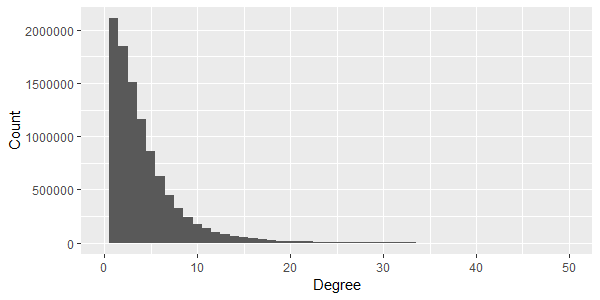
\includegraphics[width=0.85\linewidth]{degreesafter.png}
	\caption{Degree distribution after partitioning}
	\label{fig:degafter}
\end{figure}

In Figure \bref{fig:degafter} we note that the number of nodes with lower degrees has increase compared to Figure \bref{fig:degprior}. This is quite intutive since we have only removed nodes, leading to a reduction in the number of edges and as a result the average degree. We also note that the number of nodes with degrees larger than 30 are a lot fewer than in Figure \bref{fig:degprior} which is simply due to the characteristics of the partition methods which quite rapidly removes nodes of degrees larger than 20 in order to satisfy the criteria of having subgraphs of sizes lower than 1000. Degrees up to 99 exist but are very few. In Figure \bref{fig:degexp} below we can see the degree distributions before and after the partitioning together.

\begin{figure}[H]
	\centering
	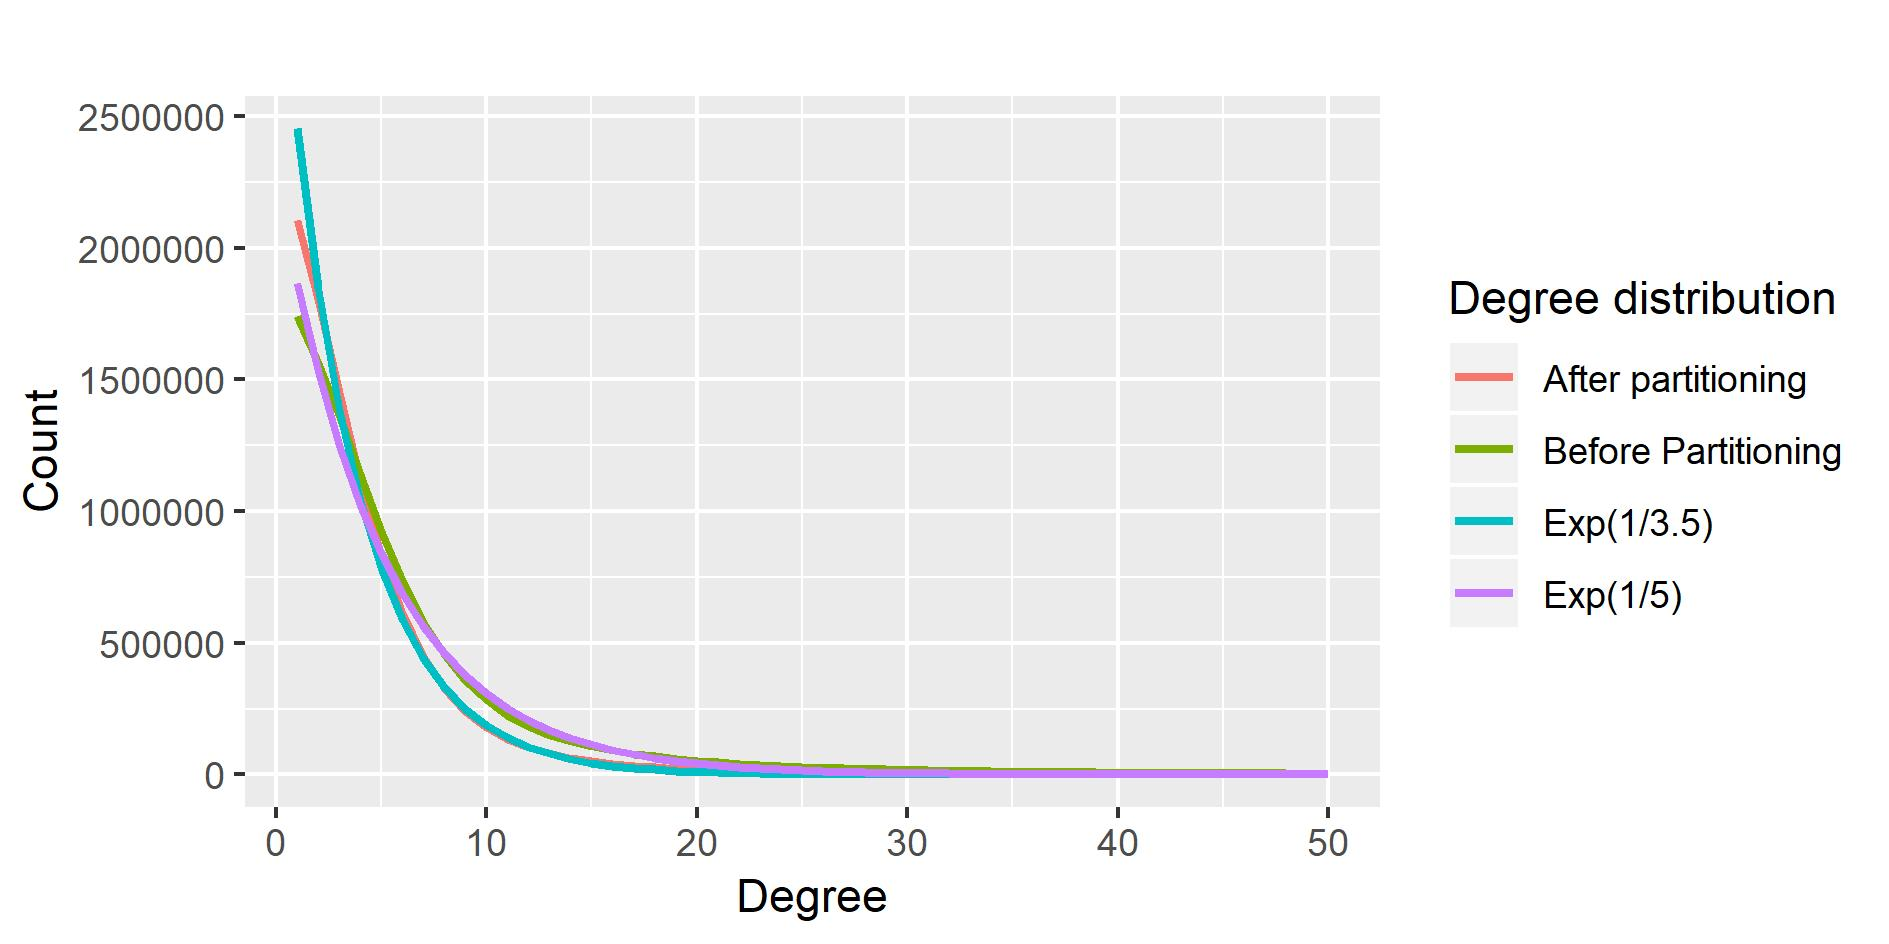
\includegraphics[width=1\linewidth]{degexp.jpeg}
	\caption{Degree distributions}
	\label{fig:degexp}
\end{figure}

Figure \bref{fig:degexp} shows that the degree distribution before and after partitioning can be described by the $Exp(1/5)$ distribution and $Exp(1/3.5)$ distribution respectively.  

If we let $D$ be the degree of a node before we partition the graph we can compute the that

$P(D>20)=e^{-20\cdot 1/5}<0.02$

$P(5<D<20)=e^{-5 \cdot 1/5}-0.02<0.35$

with the help of the fact that the degree distribution accurately seems to follow an $Exp(1/5)$ distribution for the lower degrees. We can see that nodes with degree bigger than 20 are quite unlikely but numbers between 5 and 20 are frequently occurring. This justifies our steps in the partitioning, we must be more careful for nodes with degree less than 20. One could be even more careful and checking after every node removed after some time, but we assess that this would cost a lot in time. 

\medskip

We have removed 646 394 nodes in total, 112 783 nodes with degree 100 or bigger, 191 625‬ nodes with degree between 20 and 100 and 229 203‬ between 5 and 20. Below 6 the degree distribution is the same, the increase of nodes with degree one in the plot follows from the fact that we instead of removing nodes make them isolated with degree one.

\medskip

29 179 998 edges were removed during the partitioning, we had 49 790 386 before and 20 610 388 after, meaning that we have removed more than the half of all edges. This is however reasonable since we have removed the nodes with the high degrees, in the beginning one node even had a degree close to 3 000! 

\subsection{Distribution of Disconnected Subgraphs After Partitioning}

When partitioning our graph in order to satsify the criteria we end up creating a lot more subgraphs which can be seen below.

\begin{figure}[H]
	\centering
	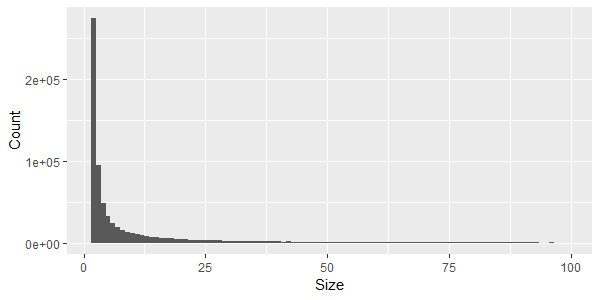
\includegraphics[width=0.85\linewidth]{sizesafter.png}
	\caption{Size distribution of the disconnected subgraphs before partitioning}
	\label{fig:sizeafter}
\end{figure}

In Figure \bref{fig:sizeafter} we actually have some noticeable number of disconnected subgraph with sizes close to $100$ which we did not have before partitioning. This is a result of partitioning the aforementioned subgraph containing 6.5 million contigs. By partitioning this graph we have also drastically increase the number of disconnected subgraph from about 486000 to about 710000, which as a result leads to increase in the number of subgraphs of smaller sizes across the board. Again notice that the x-axis is cut at Size=100, bigger sizes exist but are too few to be seen in the plot.

\bigskip


\end{document}




